\documentclass[14pt]{extarticle}
%\usepackage[14pt]{extsizes} % для того чтобы задать нестандартный 14-ый размер шрифта
\usepackage[utf8]{inputenc}
\usepackage[T1,T2A]{fontenc}
\usepackage[russian]{babel}
\usepackage{setspace,amsmath}
\usepackage[left=20mm, top=15mm, right=15mm, bottom=20mm, nohead, footskip=10mm]{geometry} % настройки полей документа
\usepackage{graphicx}
\DeclareGraphicsExtensions{.png}
\usepackage{wrapfig}
\usepackage{lipsum}
\usepackage{indentfirst}
\usepackage{longtable}
\usepackage{listings}

\lstdefinestyle{uno}{
    language=C,
    captionpos=b,
    numbers=left,
    frame=l,
    tabsize=2,
    texcl=true
}
\lstdefinestyle{python}{
    %basicstyle=\footnotesize{14}{14}\selectfont\ttfamily,
    language=Python,
    captionpos=b,
    numbers=left,
    frame=l,
    showtabs=true,
    tabsize=2,
    texcl=true
}


\begin{document} % начало документа
\renewcommand{\lstlistingname}{Пример кода}
%\renewcommand{\lstlistlistingname}{Примеры кода}

% НАЧАЛО ТИТУЛЬНОГО ЛИСТА
\begin{center}
\hfill \break
\small{\textbf{Санкт-Петербургский государственный электротехнический университет}}\\
\small{\textbf{"ЛЭТИ" им. В. И. Ульянова (Ленина)}}\\
\small{\textbf{(СПБГЭТУ "ЛЭТИ")}}\\
\hfill \break

\begin{center}
\begin{tabular}{lr}
Направление: & \textbf{27.04.04} - Управление в технических системах \\
Профиль: &  Управление и информационные технологии в технических системах \\
Факультет: & Компьютерных технологий и информатики \\
Кафедра: & Автоматики и процессов управления \\
\\
К защите допустить & \\
Зав. кафедрой &  Шестопалов М. Ю.
\end{tabular}
\end{center}

\normalsize{}
\vspace{3cm}
\large{\textbf{ВЫПУСКНАЯ КВАЛИФИКАЦИОННАЯ РАБОТА МАГИСТРА}}\\
\vspace{1cm}
\normalsize{\textbf{Тема: Параметрическое проектирование дельта-робота и решение задачи координатного управления рабочим органом}}\\
\vspace{3cm}
 
\begin{flushleft}
 \hspace{1cm} Студент \hspace{7cm} \underline{\hspace{3cm}}  О.Е. Медовиков \\ 
 \vspace{5mm}
 \hspace{1cm} Руководитель \hspace{2cm} к. т. н. \hspace{2cm} \underline{\hspace{3cm}}  С. Е. Абрамкин\\ 
 \vspace{5mm}
 \hspace{1cm} Консультант \hspace{2.3cm} к. э. н. \hspace{2cm} \underline{\hspace{3cm}}  Ю. Р. Ичкитидзе\\ 
\end{flushleft}

\vspace{2cm}
Санкт-Петербург \\ 2020 
\end{center}
\thispagestyle{empty} % выключаем отображение номера для этой страницы
 
% КОНЕЦ ТИТУЛЬНОГО ЛИСТА

\newpage
% НАЧАЛО ЗАДАНИЯ
\begin{center}
\large{\textbf{ЗАДАНИЕ НА ВЫПУСКНУЮ КВАЛИФИКАЦИОННУЮ РАБОТУ}}\\
\end{center}
\begin{flushright}
Утверждаю\\
Заф. кафедры АПУ\\
\underline{\hspace{3cm}} Шестопалов М. Ю.\\
«\underline{\hspace{0.7cm}}»\underline{\hspace{3cm}}2020 г.
\end{flushright}

\hfill \break
Студент Медовиков О. Е. \hspace{7cm} Группа 4391\\
Тема работы:\\ Параметрическое проектирование дельта-робота и решение задачи \hfill \break координатного управление рабочим органом.\\
Исходные данные (технические требования): \\
1. Написание программы для параметрического моделирования дельта-робота\\
2. Написание программы для управления дельта-роботом\\
3. Создание рабочей модели дельта-робота\\
Содержание ВКР:\\
\vspace{2cm} \\
Перечень отчетных материалов: пояснительная записка, иллюстративный\\ материал, приложение.\\
Дополнительные разделы:\\
\vspace{2cm}

\begin{tabular}{p{230pt}c}
Дата выдачи задания & Дата предоставления ВКР к защите\\
«\underline{\hspace{0.7cm}}»\underline{\hspace{3cm}}2020 г. &  «\underline{\hspace{0.7cm}}»\underline{\hspace{3cm}}2020 г.\\
\end{tabular}
\vspace{1cm}

\begin{flushleft}
 \hspace{1cm} Студент \hspace{7cm} \underline{\hspace{3cm}}  О.Е. Медовиков \\ 
 \vspace{5mm}
 \hspace{1cm} Руководитель \hspace{2cm} к. т. н. \hspace{2cm} \underline{\hspace{3cm}}  С. Е. Абрамкин\\ 
 \vspace{5mm}
 \hspace{1cm} Консультант \hspace{2.3cm} к. э. н. \hspace{2cm} \underline{\hspace{3cm}}  Ю. Р. Ичкитидзе\\
\end{flushleft}

\thispagestyle{empty} % выключаем отображение номера для этой страницы

\newpage
\begin{center}
\large{\textbf{КАЛЕНДАРНЫЙ ПЛАН ВЫПОЛНЕНИЯ ВЫПУСКНОЙ КВАЛИФИКАЦИОННОЙ РАбОТЫ}}\\
\end{center}
\begin{flushright}
Утверждаю\\
Заф. кафедры АПУ\\
\underline{\hspace{3cm}} Шестопалов М. Ю.\\
«\underline{\hspace{0.7cm}}»\underline{\hspace{3cm}}2020 г.
\vspace{1cm}
\end{flushright}

\begin{flushleft}
Студент Медовиков О. Е. \hspace{7cm} Группа 4391\\
Тема работы:\\ Параметрическое проектирование дельта-робота и решение задачи\\ координатного управление рабочим органом.\\
\vspace{1cm}
\end{flushleft}


\begin{tabular}{| c | l | c | }
\hline
№ п/п & Наименование работ & Срок выполнения\\
\hline
1 & Обзор литературы по теме работы & 10.12 - 01.02\\ 
\hline
2 & Проектирование виртуальной модели& 10.12 - 26.03\\
\hline
3 & Создание физического прототипа робота & 01.02 - 05.04\\
\hline
4 & Написание прошивки для микроконтроллера & 25.04 - 15.05 \\
\hline
5 & Создание интерфейса для управления роботом &15.05 - 25.05 \\
\hline
\end{tabular}

\vspace{3cm}

\begin{flushleft}
 \hspace{1cm} Студент \hspace{7cm} \underline{\hspace{3cm}}  О.Е. Медовиков \\ 
 \vspace{5mm}
 \hspace{1cm} Руководитель \hspace{2cm} к. т. н. \hspace{2cm} \underline{\hspace{3cm}}  С. Е. Абрамкин\\ 
 \vspace{5mm}
 \hspace{1cm} Консультант \hspace{2.3cm} к. э. н. \hspace{2cm} \underline{\hspace{3cm}}  Ю. Р. Ичкитидзе\\
\end{flushleft}

\thispagestyle{empty} % выключаем отображение номера для этой страницы


% реферат
\begin{center}
\large{\textbf{РЕФЕРАТ}}\\
\end{center}
Пояснительная записка 00 стр., 00 рис., 00 табл., 00 ист., 00 прил.\\
Ключевые слова: параметрическое моделирование, 3д печать, дельта-робот, сортировка.\\
Объект исследования:  кинематика дельта-робота.\\
Цель работы:\\
Основное содержание работы.



% аннотация на английском
\begin{center}
\large{\textbf{ABSTRACT}}\\
\end{center}
speak from my heart

% оглавление содержание
\begin{center}
\def\contentsname{СОДЕРЖАНИЕ}
\large \tableofcontents
\end{center}

\newpage

\begin{center}
    \def\lstlistlistingname{ПРИМЕРЫ КОДА}
    \large \lstlistoflistings
\end{center}
% определения (не обяз)
% введение
\addcontentsline{toc}{section}{Введение}
\begin{center}
\large{\textbf{ВВЕДЕНИЕ}}\\
\end{center}
Меня зовут дундук

% основная часть
\section{Кинематика дельта-робота}
\subsection{Конструкция и устройство}
Основанием робота является база, жёстко фиксируемая в пространстве над рабочем полем. Габариты базы очерчиваются равносторонним треугольником со стороной равной f. Середины сторон треугольника обозначают координаты осей вращения рычагов и таким образом, расстояние от центра базы до оси вращения каждого рычага равно r - радиусу вписанной окружности равностороннего треугольника. Это расстояние легко находится через соотношение:
\begin{center}
f =$\frac{\sqrt{3}}{2}$  r
\end{center}

В дальнейшей работе, при описании моделирования, будут использоваться переменные с другими названиями, например, переменная rad  соответствует радиусу вписанной окружности. Это связано с удобством написания кода, так как невозможно поиском найти переменную, обозначенную одним символом, а также это неправильно, с точки зрения читаемости кода.

\begin{figure}[h!]
	\centering
	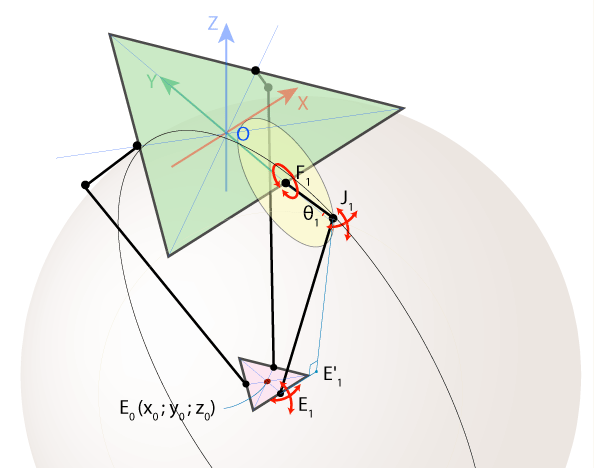
\includegraphics[width=0.8\linewidth]{./image/deltabot}
	\caption{Схематическое представление Дельта-робота}
\end{figure}

Начало координат располагается в центре базы, таким образом, чтобы Z координата высоты равнялась нулю для точек осей вращения рычагов, так как конечное расположение рабочего органа робота будет рассчитываться относительно этих координат. Три рычага нумеруются определённым образом. Первый рычаг двигается в плоскости YZ и направлен в противоположную оси Y сторону. Второй рычаг повернут относительно оси Z на 120 градусов, а третий на -120 градусов. Поворот делается по правилу правой руки, где большой палец совпадает с направлением оси Z, а согнутые пальцы показывают направление вращения. Так как робот в целом абсолютно симметричен, ошибки с нумерацией рычагов закономерны, необходимо на всех этапах строго придерживаться единому правилу обозначения рычагов.

Жёстко закреплённые каждый в своей плоскости рычаги обозначаются $r_{fi}$, а угол на который они
поворачиваются обозначают через $\theta_{i}$. Точка оси вращения рычагов обозначается как $F_{i}$, а конечная точка рычага - $J_{i}$. На конце рычага находится крепление с двумя карданными шарнирами, которое всегда параллельно стороне равностороннего треугольника, обозначающего габариты рабочего органа. Две взаимно параллельные направляющие соединяются через шарниры с вершинами треугольника, образуя параллелограмм. Из-за этого, данный робот также называют разновидностью параллельного робота.

Для математического описания робота карданные шарниры и параллельные направляющие не нужны, их заменяют рычагами обозначаемыми как $r_{ei}$. Рычаги $r_{ei}$ крепятся к серединам сторон треугольника, обозначающего габариты каретки, в которой закреплен рабочий орган. Габариты обозначаются, как и в случае с базой, равносторонним треугольником, длина стороны  которого обозначается буквой e. Координаты точек крепления карданных шарниров к каретки называют $E_{i}$, а точкой $E_{0}$ обозначается центр каретки, то-есть координата рабочего органа.

\subsection{Задача прямой кинематики дельта-робота}
Решение прямой задачи кинематики дельта-робота заключается в определении координаты центра каретки $E_{0}$ при известных углах $\theta_{i}$. Решение данной задачи необходима мне для определения координат расположения различных узлов машины, во время создания компьютерной модели. Сама идея решения достаточна проста. Так как рычаги, соединенные с двигателем, двигаются в одной плоскости, без возможности отклониться, это значит, что можно рассчитать координаты вершины рычага, зная координату оси вращения, длину рычага и угол поворота рычага. Координата конца рычагов обозначается буквой $J_{i}$. Подобным образом посчитать угол шарнира, соединяющего конец рычага и сторону каретки не представляется возможным, так как он вращается не вдоль одной плоскости, а в трёх измерениях.

Если допустить, что каретка не имеет размеров и представляет собой точку, то можно представить три сферы с центрами в $J_{i}$ и радиусами $r_{ei}$. Сферы показывают область, в которой могут теоретически могут вращаться шарниры, при данных значениях углов $\theta_{i}$. Если внести поправки на размеры каретки, точка пересечения трех сфер - будет решением, искомой координатой каретки.
\begin{figure}[h]
	\centering
	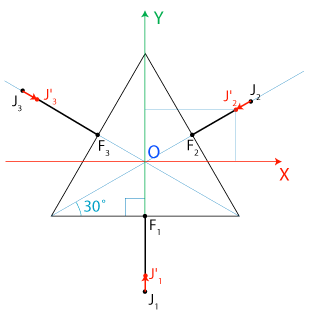
\includegraphics[width=0.4\linewidth]{./image/primay}
	\caption{Схема расчета координат рычагов}
\end{figure}

Расчет координат $J_{1}$ для первого рычага упрощается выбором системы координат. Первый рычаг параллелен оси Y и движется в плоскости YZ, поэтому координата X всегда будет равна 0. При этом Z координата оси вращения тоже равна 0, что было оговорено ранее. Значит координата $F_{1}$ будет состоять только из Y  и будет равна минус радиус вписанной окружности. В этом месте нужно взять поправку на радиус каретки, и вычесть радиус каретки из радиуса базы. Таким образом, мы сможем рассчитать точки  $J'_{i}$ - центры сфер, с общей точкой в $E_{0}$. 
\begin{center}
$t = r_{base} - r_{karet}$\\
$J'_{1} = (x_{1};y_{1};z_{1})$\\
$J'_{2} = (x_{2};y_{2};z_{2})$\\
$J'_{3} = (x_{3};y_{3};z_{3})$\\
\begin{equation*}
 \begin{cases}
        x_{1} = 0 \\
        y_{1} = -(t - r_{f}cos(\theta_{1})) \qquad\\
        z_{1} = -r_{f}cos(\theta_{1})\\
    \end{cases}
\end{equation*}
\begin{equation*}
    \begin{cases}
        x_{2} = [t+r_{f}cos(\theta_{2})]cos(30^{\circ})\\
        y_{2} = [t+r_{1}cos(\theta_{2})]sin(30^{\circ})\\
        z_{2} = -r_{f}sin(\theta_{2})\\
    \end{cases}    
\end{equation*}
\begin{equation*}
    \begin{cases}
        x_{3} = [t+r_{f}cos(\theta_{3})]cos(30^{\circ})\\
        y_{3} = [t+r_{1}cos(\theta_{3})]sin(30^{\circ})\\
        z_{3} = -r_{f}sin(\theta_{3})\\
    \end{cases}    
\end{equation*}
\end{center}

Теперь для нахождения координаты каретки, нужно решить систему из трех уравнений сфер с координатами центров в $J'_{i}$ и радиусами $r_e$.
\begin{center}
    $E_{0} = (x,y,z)$
    $( x - x_{i} )^{2} + ( y - y_{i} )^{2} + ( z - z_{i} )^{2} = r^{2}_{e} $
\end{center}

Подставим координаты $J'_{i}$, полученные ранее и получим систему уравнений вида:

\begin{equation*}
    \begin{cases}
        x^{2} + (y - y_{1})^{2} + (z - z_{1})^{2} = r^{2}_{e}\\
        (x - x_{2})^{2} + (y - y_{2})^{2} + (z - z_{2})^{2} = r^{2}_{e}\\
        (x - x_{3})^{2} + (y - y_{3})^{2} + (z - z_{3})^{2} = r^{2}_{e}\\
    \end{cases}    
\end{equation*}

Теперь раскроем скобки и немного сгруппируем переменные:

\begin{equation*}
    \begin{cases}
x^{2} + y^{2} + z^{2} - 2y_{1}y - 2z_{1}z = r^2_{e} - y^2_{1} - z^2_{1}\\
x^{2} + y^{2} + z^{2} - 2x_{2}x - 2y_{2}y - 2z_{1}z = r^2_{e} - x^2_{2} - y^2_{2} - z^2_{2}\\
x^{2} + y^{2} + z^{2} - 2x_{3}x - 2y_{3}y - 2z_{1}z = r^2_{e} - x^2_{3} - y^2_{3} -z^2_{3}\\
    \end{cases}    
\end{equation*}

Теперь можно сделать подстановку и формируем новые три уравнения, вычитая из первого сначала второе, потом третье и из второго - третье.
\begin{center}
    $\omega_{i} = x^2_{i} + y^2_{i}  + z^2_{i} $
\end{center}

\begin{equation*}
    \begin{cases}
x_{2}x + (y_{1} - y_{2})y + (z_{1} - z_{2})z = (\omega_{1} - \omega_{2})/2 \\
x_{3}x + (y_{1} - y_{3})y + (z_{1} - z_{3})z = (\omega_{1} - \omega_{3})/2 \\
(x_{2} - x_{3})x + (y_{2} - y_{3})y + (z_{2} - z_{3})z = (\omega_{2} - \omega_{3})/2 \\
    \end{cases}    
\end{equation*}

Следующим шагом вычитаем второе уравнение из первого, частично сократив $y$ выразив $x$ через $z$. Аналогично вычитаем из второго третье, частично сокращая $x$ и выражая $y$ через $z$. Так как выражения получаются очень длинными, для компактной записи вводится подстановка $a_{i},b_{i},d$.
\begin{center}
$x = a_{1}z+b_{1} \qquad  y=a_{2}z+b_{2}$\\
\end{center}

\vspace{0.75cm}
\hspace{4cm} $a_{1} =\frac{1}{d}[(z_{2}-z_{1})(y_{3}-y_{1})-(z_{3}-z_{1})(y_{2}-y_{1})]$

\hspace{4cm} $b_{1} =-\frac{1}{2d}[(\omega_{2}-\omega_{1})(y_{3}-y_{1})-(\omega_{3}-\omega_{1})(y_{2}-y_{1})]$\\
\vspace{0.75cm}

\hspace{4cm} $a_{2} =-\frac{1}{d}[(z_{2}-z_{1})x_{3}-(z_{3}-z_{1})x_{2}]$

\hspace{4cm} $b_{2} =\frac{1}{2d}[(\omega_{2}-\omega_{1})x_{3}-(\omega_{3}-\omega_{1})x_{2}]$

\vspace{0.75cm}
\hspace{4cm} $d=(y_{2}-y_{1})x_{3} - (y_{3}-y_{1})x_{2}$\\
\vspace{0.75cm}

Теперь, имея $x$ и $y$, выраженные через $z$, предстоит подставить их в уравнение сферы (например, первой) с центром в $J_{1}$, раскрыть скобки, упростить и получить:

\begin{center}
$(a^{2}_{1}+a^{2}_{2}+1)z^{2} + 2(a_{1}+a_{2}(b_{2}-y_{1})-z_{1})z +(b^{2}_{1}+(b_{2}-y_{1})^2 +z^{2}_{1}-r^{2}_{e})=0$
\end{center}

В конечном итоге задача свелась к решению квадратного уравнения, через дискриминант, корни которого будут равны $Z$ координате каретки. На данном этапе проводится проверка параметров дельта-робота. Человек произвольно задающий радиусы базы и каретки, длины рычагов и шарниров должен подобрать их в определённом соотношении, которое позволит роботу физически функционировать. Иначе, шарниры будут слишком короткими и не дотянутся до каретки. Решение уравнения выше позволяет определить физическую возможность создания робота при данных параметрах. Если дискриминант равен отрицательному числу, значит, что шарниры не дотягиваются до каретки и поэтому выбор параметров робота неверен. Если дискриминант равен 0 в рабочей области робота это приводит к неустойчивому равновесию. Эта координата называется точкой сингулярности параллельного робота, так как в её окрестностях находятся координаты с двумя равнозначными и очень близкими решениями. В окрестностях точки сингулярности управление роботом практически невозможно, так как движение вверх или вниз по оси $Z$ будет случайным. Некоторые конструкции параллельных роботов, проходя точку сингулярности, "защёлкиваются" в положение, из которого не могут выйти самостоятельно. Для правильной работы робота дискриминант должен быть большим числом, в случае моей симуляции числа достигают значений $1.4*10^{25}$ и даже больше.

\subsection{Обратная кинематика}

Задача обратной кинематики дельта-робота заключается в нахождении углов поворота рычагов $\theta_{i}$, при известной координате каретки $E_{0}=(x_{0},y_{0},z_{0})$. Данное решение основано на нахождении координат деталей первого шарнира и рычага, и вывода решения для угла $\theta_{1}$ в общем виде для первого рычага с учётом правильного расположения осей координат. Два оставшихся угла будут рассчитаны аналогично, с применением вращения оси координат на $120^{\circ}$ и $-120^{\circ}$ соответственно.

Первым шагом необходимо найти координаты крепления шарнира к каретке. Эта точка находится на стороне равностороннего треугольника и смещена от точки $E_{0}$ на величину радиуса вписанной окружности.

\begin{center}
$E_{1} (x_{0},y_{0}-\frac{e}{2\sqrt{3}},z_{0})$
\end{center}

Так как в общем виде каретка будет иметь некое смещение по оси $X$, а это значит, что шарнир и рычаг не будут лежать в одной плоскости $YZ$. Для решения необходимо найти проекцию шарнира на плоскость $YZ$. Верхняя точка проекции шарнира совпадает с координатой конца рычага $J_{1}$, а нижняя точка обозначается $E'_{0}$. 

\begin{center}
$E'_{1} (0,y_{0}-\frac{e}{2\sqrt{3}},z_{0})$
\end{center}

Соответственно длинна проекции шарнира находится по теореме Пифагора:

\begin{center}
$E'_{1}J_{1} = \sqrt{(E_{1}J_{1})^{2} -(E_{1}E'_{1})^{2}}  $
\end{center}

Так как гипотенуза равна длине шарнира, а меньший катет - смещению каретки по $X$, то: 

\begin{center}
    $E'_{1}J_{1} = \sqrt{r^{2}_{e} - x^{2}_{0} }  $
\end{center}

Напомню, что координата оси вращения первого рычага $F_{1}$  смещена от центра координат на радиус вписанной окружности, таким же образом, как и крепление шарнира каретки.

\begin{center}
    $F_{1}(0,\frac{-f}{2\sqrt{3}},0)$
\end{center}

Теперь есть все необходимое, для нахождения координаты соединения рычага с шарниром $J_{1}$. Вращаясь рычаг описывает окружность с радиусом $r_{f}$ и центром в  $F_{1}$. Проекция шарнира вращаясь описывает окружность с найденным выше радиусом $E'_{1}J_{1}$ и центром в $E'_{1}$. Найдя точки пересечения этих двух окружностей, мы получим две физически возможные координаты точки соединения рычага и шарнира, одна из которых ложная, а вторая (наименьшая по $Y$) истинная. Общие точки находятся путём решения решения системы уравнений двух окружностей.

\begin{equation*}
    \begin{cases}
        (y_{J_{1}} -y_{F_{1}})^{2} +(Z_{J_{1}}-z_{F_{1}})^{2} = r^{2}_{f}\\
        (y_{J_{1}} -y_{E'_{1}})^{2} +(Z_{J_{1}}-z_{E'_{1}})^{2} = r^{2}_{e}-x_{0}\\
    \end{cases}
\end{equation*}

Подставляем известные координаты центров окружностей:


\begin{equation*}
    \begin{cases}
        (y_{J_{1}} + \frac{f}{2\sqrt{3}})^{2} + z^{2}_{J_{1}} = r^{2}_{f}\\
        (y_{J_{1}} -y_{0} +\frac{e}{2\sqrt{3}})^{2} +(z_{J_{1}} -z_{0})^{2} = r^{2}_{e}-x_{0}\\
    \end{cases}
\end{equation*}

 В данном случае, так как мы работаем с окружностями и игнорируем ось $X$, получается система из двух уравнений с двумя неизвестными. Если раскрыть скобки и вычесть из первого уравнения второе, то можно выразить $z$ через $y$ и подставить во второе уравнение, получив квадратное уравнение.

 \begin{center}
\vspace{0.75cm}
 $\frac{x^{2}_{0}+y^{2}_{0}+z^{2}_{0}+r^{2}_{e}+r^{2}_{f} -y^{2}_{F_{1}} }{2z_{0}}y^{2} - \frac{y_{F_{1}}-y_{0}}{z_{0}}y = 0$
\end{center}







\section{Моделирование робота}
\subsection{База}
бла бла

\section{Программирование Arduino}
\subsection{Драйвера двигателей}

Для управления шаговыми двигателями используют платы-драйвера, в моем случае это самые распространенные А4988. Их функция заключается в формировании псевдосинусоидальных токов в обмотках шагового двигателя, заставляя его делать шаги или микрошаги. Благодаря подаче сигналов на контакты MS1, MS2, MS3 можно выставить дробление шага от $\frac{1}{2}$ до $\frac{1}{32}$. Дробление шага позволяет увеличить в разы точность позиционирования, путем увеличения количества шагов на оборт, но от этого страдает скорость вращения и момент. В данном проекте, скорость и момент важнее точности, поэтому функция дробления шага не была задействована.

Управление драйвером происходит с помощью трех контактов. Первый, отвечает за включение (enable), без подачи напряжения на этот конакт, драйвер будет игнорировать команды на движение. Наличие сигнала на контакте dir определяет направление последующих шагов. Каждый сигнал на контакте step является командой драйверу сделать шаг двигателем.    

Питание на драйвер приходит в обход платы Arduino, в моем проекте используется 12-ти вольтовый адаптер питания. Если отключить обмотки двигателя, то можно настроить ток драйвера, вращая отверткой потенциометр на плате. Для разных драйверов токи считаются по-своему, в случае с А4988 она выглядит так:

\begin{center}
$I_{raschet} = \frac{I_{nominal\_dvig}}{2.5} = \frac{1.7}{2.5} = 0.68 A $
\end{center}

\begin{figure}[h]
\centering
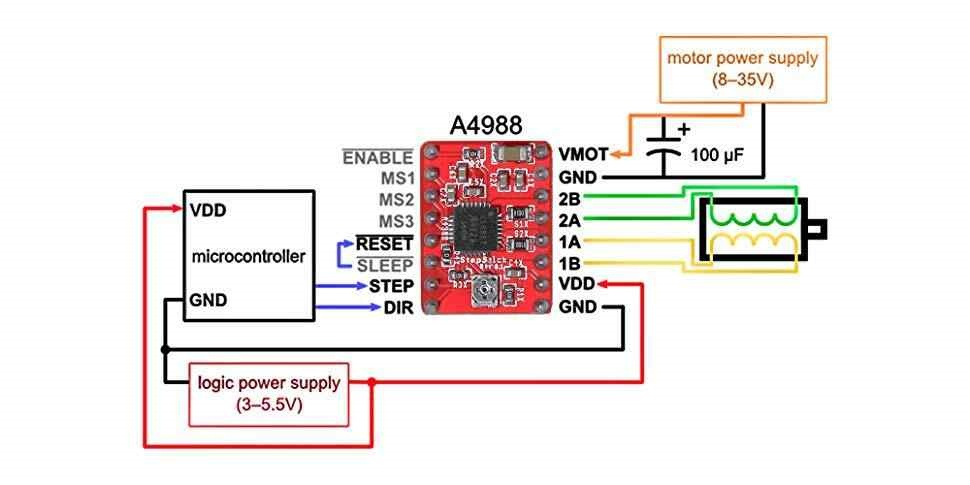
\includegraphics[width=0.8\linewidth]{./image/a4988}
\caption{Схема контактов драйвера шагового двигателя}
\end{figure}

Выставленное значение тока влияет на момент, с которым работает двигатель, на его шумность и силу нагрева. При завышении токов можно увеличить момент, но нагреть двигатель до $90^{\circ}$, что может размягчить пластик, который не держит температуры выше $80^{\circ}$. Занижение токов приведет к понижению шума, вибраций и температуры, но двигатель может начать пропускать шаги из-за недостаточного момента. 

\subsection{Распиновка Arduino CNC Shield}

Arduino CNC Shield продается как готовое решение для самодельных трехосевых станков. Плата создана специально под открытую прошивку GRBL для Arduino. Для взаимодействия с этой прошивкой энтузиасты написали несколько программ для различного использывания CNC станков (фрезеровка, графировка или рисование). Общение с платой происходит с помощью команд gcode, отправляемых по com-порту. Поддерживаются функции плавного набора скорости шаговых двигателей, плавное движение по окружностям и спиралям и другие возможности.

Тем не менее специфика движения дельта-робота заключается в том, что все 3 шаговых двигателя должны работать одновременно. В то время, как в линейных станках одновременно работают только две оси и только в предварительно заложенных функциях, например, по рисованию окружностей. С помощью gcode можно управлять углами поворотов рычагов, через координаты x, y, z. Но нужно понимать, что внутри программы будут одновременно переменные x, y, z, которые обозначают координату в пространстве и x, y, z, которые являются углами.   

\begin{figure}[h]
\centering
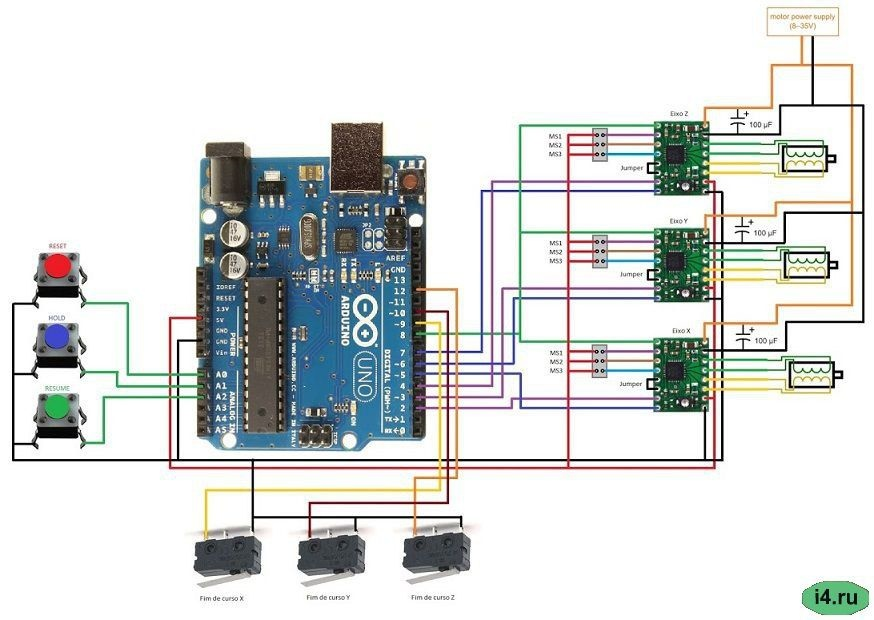
\includegraphics[width=0.8\linewidth]{./image/shield}
\caption{Схема распиновки Arduino CNC Shield}
\end{figure}

В качестве тренировки и для набора практического навыка, решил самостоятельно написать скетч. Первым делом необходимо объявить рабочие пины Arduino:

\begin{lstlisting}[style=uno,caption=Объявление пинов Arduino]
int step1 = 2;
int step2 = 3;
int step3 = 4;

int dir1 = 5;
int dir2 = 6;
int dir3 = 7;

int pwr = 8;

int kon1 = 9;
int kon2 = 10;
int kon3 = 11;

void setup() {
  Serial.begin(115200);
  pinMode(step1, OUTPUT);
  pinMode(step2, OUTPUT);
  pinMode(step3, OUTPUT);
  pinMode(dir1, OUTPUT);
  pinMode(dir2, OUTPUT);
  pinMode(dir3, OUTPUT);
  pinMode(pwr, OUTPUT);
  pinMode(kon1, INPUT);
  pinMode(kon2, INPUT);
  pinMode(kon3, INPUT);
  }

\end{lstlisting}

Я создаю переменные, обозначающие номер порта, чтобы иметь возможность в случае необходимости менять порт, не переписывая код скетча целиком. Порты с 2 по 8 назначаю выходами и с помощью них буду отправлять управляющие сигналы на драйвера. Порты с 9 по 11 назначаются входами, в случае если в процессе выполнения движения рычаг нажмет на концевик, то на один из этих портов придет сигнал. К сожалению, оба концевика: минимальное положение и максимальное положение, у данной паты выведены на 1 пин. Поэтому определить, какой именно концевик сработал можно только по направлению движения двигателя.  


\subsection{Основная функция}

Под основной функцией в скетче подразумевается управление Arduino с помощью команд, принимаемых через com-порт. Так как ком порт ограничен тем, что мы можем отправлять только восьмибитные сообщения, представляющие собой число от 0 до 256, конвертируемое в символ ASCI кодировки, то и команды представляют собой 1 символ. Для передачи числа в формате Int, представляющее собой 4 байта, необходимо со строны компьютера разбить перменную Int на массив из 4 символов float, и передовать их по очереди. Со стороны Arduino существует функция Serial.parseInt, которая собирает 4 символа float, обратно в переменную типа Int. На данный момент, я ограничился двумя командами: возврат каретки в исходную позицию и перемещение каретки в новую координату. Начальная позиция в даннном случае это углы $\theta_{i}$ равные $-15^{\circ}$. Углы необходимо перевести в шаги двигателей и работать с ними.
\begin{center}
    $n_{shagov} = \frac{\theta_{max} - \theta_{min} }{360^{\circ}}* N_{dvig} * K_{reductor} = \frac{90^{\circ}+15^{\circ}}{360^{\circ}}*200*6 = 350$
\end{center}

Количество шагов от минимального до максимального положения является отношением полного угла к полной окружности, домноженное на количество шагов на оборот шагового двигателя и на коэффицент передачи редуктора. Получается, что для прохождения рычага до крайнего положения необходимо сделать 350 шагов, что больше 256, поэтому мы не можем использовать 8 битные числа для передачи изменения координаты, а вынуждены использовать переменные типа Int.

Для того, чтобы узнать на какие углы необходимо переместить рычаги необходимо дважды решить решить обратную задачу управления. Первый раз мы рассчитываем углы $\theta_{i}$ для настоящего положения в пространстве, а второй раз для последующего положения. И только вычитая результат первого решения из второго, мы получим значение изменения углов. 
В скетче ардуино, я завожу 9 переменных, отвечающих за хранение состояния углов: текущие значение $\theta_{i}$, новые значения, полученные по com-порту, и $\Delta_{i}$, разница между ними. 

Плата Arduino в бесконечном цикле ожидает сигнала по com-порту. Если будет получена буква H, что обозначает home, то будет вызвана функция move\_home(). Важно, что именно перед вызовом функции движения, я отключаю порт pwr, тем самым разрешая работу драйверам. После выполнения функции двиения, возвращаем драйверам запрет на движение и посылаем в com-порт букву Y, подтверждение для компьютера, что функция выполнена адекватно

Если получена буква С, что обозначает change position, Arduino по очереди запрашивает значение координат, в которые необходимо перенести каретку. Происходит расчет $\Delta_{i}$, снимается запрет на работу драйверов и выполняется функция движения каретки.

Подсчет текущего значения углов $\theta_{i}$ будет происходить внутри функций движения.
\begin{lstlisting}[style=uno,caption=Основная функция скетча]
void loop() {
    if (Serial.available() > 0) {

        val = Serial.read();
        Serial.write(val);

        if (val == 'H') { 
            digitalWrite(pwr,LOW);
            move_home();
            digitalWrite(pwr,HIGH);
            Serial.print('Y');}

        if (val == 'C') {
            Serial.print('X');
            NEW_teta1 = Serial.parseInt();
            Serial.print('Y');
            NEW_teta2 = Serial.parseInt();
            Serial.print('Z');
            NEW_teta3 = Serial.parseInt();
            
            delta1 = NEW_teta1 - teta1;
            delta2 = NEW_teta2 - teta2;
            delta3 = NEW_teta3 - teta3;
            
            digitalWrite(pwr,LOW);
            change_location();
            digitalWrite(pwr,HIGH);

            Serial.print('Y'); 

            }
    }
}
\end{lstlisting}

\subsection{Функция возврата каретки домой}

Функция возврата каретки домой устроена по принципу, движения двигателя до тех пор, пока не появится сигнал на соответсвующем порту, к котрому подключен концевик. Цикл while выполняется до тех пор пока все концевики не будут активированы. В условии использованно логическое ИЛИ и утверждение, что концевики в неактивированном состоянии. Пока хоть один из них будет неактивирован, цикл будет выполняться. Внутри цикла происходит дополнительная проверка на концевики для каждого двигателя, перед выполнением функции движения. Это делается потому, что скорее всего рычаги придут в крайние положения не синхронно.

После выполнения цикла, все рычаги должны оказаться в начальной позиции, соответсвенно можно обнулить глобальные переменные текущих значений $\theta_{i}$.

\begin{lstlisting}[style=uno,caption=Функция возврата каретки домой]
int move_home(){
    while(digitalRead(kon1)==LOW|| //неправильный перенос строки
            digitalRead(kon2)==LOW||
                digitalRead(kon3)==LOW){
        if(digitalRead(kon1)==LOW){move_teta1(-1);}
        if(digitalRead(kon2)==LOW){move_teta2(-1);}
        if(digitalRead(kon3)==LOW){move_teta3(-1);}
        }
    teta1 = 0;
    teta2 = 0;
    teta3 = 0;
}
\end{lstlisting}

Функции изменения угла рычага однотипны, создают два сигнала на нужные выходы, с некоторой задержкой. В зависимости от необходимого направления движения, задается положительное или отрицательное k. В зависимости от знака, на пин dir либо подается, либо не подается напряжение. После подачи сигнала на направление, необходимо дать задержку, в данном случае это t миллисекунд. После подачи сигнала step, делается вторая задержка для совершения шага. Величины задержек зависят от скорости срабатывания платы микроконтроллера. Для драйвера A4988 задержки очень большие, двигатель не может начать движение, если задать их меньше 500 микросекунд. Это связано с резким спадом момента на роторе, так как управляющий ток не успевает нарастать за такой промежуток времени. Если уменьшать задержки уже вращающегося двигателя, то можно плавно опустить их до 250 микросекунд, но при любом толчке происходит пропуск шагов и двигатель останавливается. Так как мне важна стабильная работа двигателей, без пропуска шагов и с хорошим моментом, я решил использовать задерки в 1 миллисекунду. В своем предыдущем проекте, когда использовал трехканальный драйвер SMD-303 совсем другой ценовой категории, то использовал задержки в 50-60 микросекунд. Этот опыт оказался вредным, так как выставляя низкие задержки, я потратил много времени, считая что двигатели не могут повернуть редуктор, так как клинит шестерни. Я повышал задержки до 200 микросекунд, но это не давало результата, я пересобирал конструкцию, печатал новые шестеренки и тратил время и силы впустую.   

\begin{lstlisting}[style=uno,caption=Функция управляющяя шаговым двигателем]
int move_teta1(int k){
    if (k>0) {
    digitalWrite(dir1,HIGH);
    delay(t);
    digitalWrite(step1,HIGH);
    delay(t);
    teta1++; }
    if (k<0) {
    digitalWrite(dir1,LOW);
    delay(t);
    digitalWrite(step1,HIGH);
    delay(t);
    teta1--; }
}
\end{lstlisting}

\subsection{Функция изменения координаты}

Логика данной функции заключается в поочередном совершении шагов двигателями до тех пор, пока разница в координатах $\Delta_{i}$ не станет равной нулю. Цикл while выполняется тогда, когда есть отличная от нуля разница в координатах. Используется логическое ИЛИ. Внутри цикла происходит повторная проверка, что разница не равно нулю и одновременно не задействованны концевики. После этого, в зависимости от знака разницы, вызывается функция движения в определенную сторону, а разница уменьшается по модулю на единицу. Если разница по одной из координат станет равной нулю раньше остальных или будет задействован концевик, этот двигатель прекратит движение и будет ждать остальных. В случае, если рычаг активировал концевик до того, как разница стала нулевой, то на этот случай происходит обнуление разницы, чтобы цикл не превращался в бесконечный.

\begin{lstlisting}[style=uno,caption=Функция изменения координаты]
int change_location(){
    while(delta1 != 0||delta2 != 0||delta3 != 0){
        if( delta1 !=0 && digitalRead(kon1)==LOW) {
            if( delta1 > 0 ) {move_teta1(1); delta1--;}
            else {move_teta1(-1); delta1++;}}
        else{delta1 = 0;}
        if( delta2 !=0 && digitalRead(kon2)==LOW) {
            if( delta2 > 0 ) {move_teta2(1); delta2--;}
            else {move_teta2(-1); delta2++;}}
        else{delta2 = 0;}
        if( delta3 !=0 && digitalRead(kon3)==LOW) {
            if( delta3 > 0 ) {move_teta3(1); delta3--;}
            else {move_teta3(-1); delta3++;}}
        else{delta3 = 0;}
    }
}
\end{lstlisting}

Слабое место данной функции в том, что двигатели поочередно делают шаги. Один шаг занимает 2 миллисекунды, а это значит, что пока один двигатель двигается, два других будут проставивать в течение 4 миллисекунд. Эксперементируя с данным скетчем, в какой-то момент я придумал, каким образом надо изменить функцию, чтобы двигатели двигались действительно одновременно. Изначально, мне не удавалось победить то обстоятельство, что у каретки есть шесть степеней свободы, что подразумевает необходимость написания шести разных функций, но решение нашлось.

В новой функции нет вызова других функции управления двигателями, так как это оказалось ненужным. Цикл while как и в прошлый раз выполняется до тех пор, пока хоть одна из переменных $Delts_{i}$ отлична от нуля. Внутри цикл делится на две половины. В первой половине, в зависимости от знака разницы посылаются сигналы dir, отвечающие за направление движения. Если разница равна нулю, сигнал будет послан, но к ошибке это не приведет. После этой операции происходит необходимая задержка. Во второй половине цикла происходит проверка на отличие разницы от нуля и срабатывание концевика. Если разница отлична от нуля и концевик не сработал, то можно отправлять сигнал на шаг. После чего остается только изменить глобальное значение угла и разницы на единицу. Если сработал концевик, но разница при этом не равна нулю, она приравнивается к нулю, чтобы цикл while не становился бесконечным.  

Таким образом мне удалось реализовать одновременное функционирование двигателей, в независимости от направления движения и разнице количества шагов. Более того, так как двигатели работают одновременно и имеют общую задержку, ее можно очень просто менять во времени, тем самым разгоняя двигатели. В моем случае, драйвера очень плохо реагируют на разгон, поэтому я меняю задержку с 1000 микросекунд до 500 микросекунд в течение 22 шагов, по квадратичному закону. Возможно, дальнейшие эксперименты позволят выжать из драйверов большие показатели, возможно стоит завысить токи, но это требует дальнейших испытаний. И важно придумать способ отлавливать пропущенные шаги, так как двигатель иногда может пропускать шаги без остановок, но отследить это без обратной связи невозможно.

\begin{lstlisting}[style=uno,caption=Усложненная функция с плавным разгоном]
int hard_change_location(){
    int k = 0;
    while(delta1 != 0||delta2 != 0||delta3 != 0){

        if(del2ta1 > 0) {digitalWrite(dir1,HIGH);}
            else {digitalWrite(dir1,LOW);}
        if(delta2 > 0) {digitalWrite(dir2,HIGH);}
            else {digitalWrite(dir2,LOW);}
        if(delta3 > 0) {digitalWrite(dir3,HIGH);}
            else {digitalWrite(dir3,LOW);}

        delayMicroseconds(1000 - k*k);

        if(delta1 !=0 && digitalRead(kon1)==LOW) {
            digitalWrite(step1,HIGH);
            if(delta1 > 0) {delta1--; teta1++;}
                else{delta1++; teta1--;}}
        else {delta1=0;}

        if(delta2 !=0 && digitalRead(kon2)==LOW) {
            digitalWrite(step2,HIGH);
            if(delta2 > 0) {delta2--; teta2++;}
                else{delta2++; teta2--;}}
        else {delta2=0;}

        if(delta3 !=0 && digitalRead(kon3)==LOW) {
            digitalWrite(step3,HIGH);
            if(delta3 > 0) {delta3--; teta3++;}
                else{delta3++; teta3--;}}
        else {delta3=0;}

        delayMicroseconds(1000 - k*k);

        if (k < 22) {k++;}
    }
}
\end{lstlisting}

\subsection{Вывод}

Данным скетчем реализован минимальный функционал, необходимый для управления роботом. Arduino умеет возвращать каретку в начальное положение, отсчитывать координаты, и перемещаться на заданные через com-порт величины углов. Важно, что благодаря реализованной фунции, двигатели совершают шаги единовременно, без простоя. Есть пространство для улучшения механизма разгона двигателей, возможно, получится реализовать дополнительно торможение по квадратичному закону.Ощущается упор в возможности драйвера a4988, возможно стоит расмотреть другие варианты драйверов.  


\section{Программирование интерфейса}
\subsection{Выбор среды разработки}

Первоначально интерфейс для работы с дельта-роботом предполагалось написать на основе Qt5 в среде разработки QtCreator. У меня были первоначальные наработки, связанные с предыдущим проектом фрезерного станка на Arduino. Планировалось использовать уже написанные ранее функции передачи данных через последовательный порт, для управления платой микроконтроллера. Тем не менее из-за некоторых проблем, связанных с регистрацией лицензии пробной версии QtCreator и внезапной невозможности сборки старого проекта (необходимо соблюдать версии IDE, компилятора и библиотек). Было принято решение полностью отказаться от Qt и использовать для написания интерфейса другую технологию.

В конечном итоге программа была написано с нуля на Python с применением библиотеки создания простых интерфейсов PySimpleGui. Данная библиотека идеально подходит для создания простых интерфейсов программ, без использования сторонних сред разработки. Существуют другие подобные аналоги, в частности Tkinter, который позволяет реализовать все стандартные виджеты, которые используются в интерфейсах программ:  кнопки, текстовые поля для ввода, надписи, скроллеры, списки, радиокнопки, флажки и другие. Но вариант PySimpleGui показался более интуитивно понятным. Не смотря на то, что у обоих вариантов есть свои "поваренные книги" с различными готовыми примерами стандартных окон, которые необходимо просто адаптировать под собственные нужды. Радует простота создания графического интерфейса, в предалах одного рабочего скрипта достаточно объявить библиотеку и в дальнейшем можно генерировать окна приложения обычными вызывами функций таким образом, каким это требуется. Простой интерфейс подразумевает, что у вас нет каталогизированного проекта, состоящего из различных по функционалу файлов. Есть только скрипт с необходимостью в определенный момент создать окно с несколькими стандартными виджетами, что реализуется несколькими строками кода.  

Хорошей особенностью PySimpleGui является наличие легко настраиваемых тем. Во-первых, существует несколько десятков стандартных тем, которые можно оценить, создав тестовый скрипт и прописав команду sg.theme\_previewer(). После запуска будут сгенерированны тестовые окна со всеми стандартными темами. В итоге, не нужно поочередно менять своему проекту все возможные варианты тем, а можно сразу подобрать самую привлекательную. В моем случае - DarkAmber. Подобный простейший функционал попросту отсутсвует в Qt Designer, так как подразумевается, что в коммерческом проекте дизайн будет профессиональным, разработанным с нуля и будет представлять некоторую стоимость с точки зрения авторского права. Но для решения простых, прикладных задач данный подход чрезвычайно трудоемок.

\subsection{Интерфейс программы}

Основная цель интерфейса программы - это удобная визуализация в одном месте всех переменных, которые используются внутри скрипта и обратная связь с пользователем. Для обратной связи служит многостроковое поле для текста, в котором выводятся сообщения о выполненных действиях скрипта. Я старался делать как можно больше сообщений, в самых критических местах, чтобы иметь возможность видеть на каких этапах произошел сбой. К сожалению, мне не удалось сделать вывод об ошибке о несуществующем последовательном порте, так как подобная проверка приводит к вылету программы с ошибкой о несуществующем порте. Вообще достаточно сложно программировать последовательный порт, из-за самых разных возникающих проблем. Для простоты, я решил предположить, что пользователь знает имя последовательного порта, по которому подключен микроконтроллер и в данном месте не делать проверок.

\begin{figure}[h!]
\centering
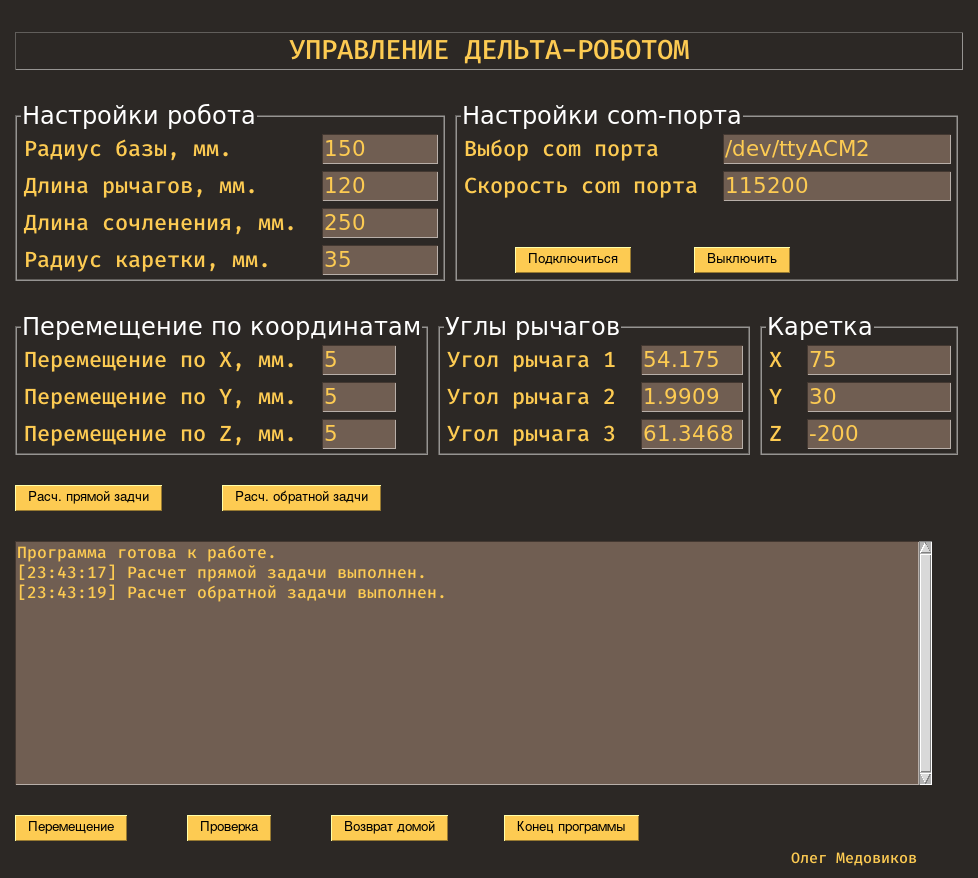
\includegraphics[width=0.8\linewidth]{./image/gui}
\caption{Интерфейс программы управления дельта-роботом}
\end{figure}

Интерфейс состоит из нескольких блоков переменных, которые разделены логически и визуально, как и в графическом виде, так и внутри скрипта, для простоты работы и пользователя и программиста. 


\begin{lstlisting}[style=python,caption=Использование PySimpleGui]

import PySimpleGUI as sg

sg.theme('DarkAmber')   # Цветовая схема

layout = [ # Наполнение окна: текстовое поле и кнопка
[sg.Text('Oleg',font=("Fira Code",16)), sg.Button('Example')],
            ]

while True:  # Цикл вызова окна
    event, values = window.read()

    if event == 'Example':   # Действие при нажатии 
        primaiaZadacha()


window.close()
\end{lstlisting}

Наполнение окна виджетами записывается в виде двойного массива $layout = [ [witget1], [witget2]]$. Для создания блоков, формируются особые виджеты фреймы, которые можно расписывать аналогично, в виде двойного массива виджетов.В минус данной библиотеки можно записать то, что по умолчанию используется не квадратный шрифт, возможно, подхватывается какой-то из системных шрифтов. Не квадратный шрифт подразумевает, что разные буквы могут иметь разную ширину в пикселях. Так как расположение полей ввода регулируется с помощью текстового блока слева, с таким шрифтом их невозможно расположить ровно, если надписи разные. Поэтому я использовал шрифт Fira Code.

\subsection{Поля с переменными движения}

При расчете параметров движения используются поля, где указаны главные параметры дельта-робота в миллиметрах. Все параметры интерактивны и функции расчета движения каждый раз берут именно те значения, которые в данный момент отображены в полях. По умолчанию в полях отображаются значения робота, воплощенного в експериментальной модели.


Поля <<Перемещение по координатам>> необходимы для ввода значений, на которое требуется изменить коодинаты каретки робота. Поля используются только для работы кнопки <<Перемещение>>. Логика программы подразумевает, что пользователь апперирует координатами, а микроконтроллер углами рычагов. Поэтому, когда пользователь заносит требуемое изменение координат в миллиметрах, программа решает обратную задачу управления и получает углы, соответсвующие этим координатам. Углы нормализуются, переводятся в шаги шаговых двигателей и отправляются в  Arduino, которая заставляет двигатели совершить нужное количество шагов.

Поля <<Углы рычагов>> и <<Каретка>> отображают значение углов рычагов в градусах и координаты каретки в миллиметрах. Данные поля используются функциями расчета прямой и обратной задачи, которые берут из них значения и обновляют при завершении расчетов.

\begin{lstlisting}[style=python,caption=Получение и обновление значения виджета]
frame_delta = [
    [sg.Text('Number',font=("Fira Code",16)),
    sg.InputText('150',size=(8,1),font='any 16',key='value')],
                ]

N  = float(values['value'])

N = N + S

 window['value'].update(str(round(N,2)))
\end{lstlisting}

Получить значение из виджета можно при условии, что указан ключ - показатель данного значения. Необходимо помнить, что значение внутри виджета всегда будет иметь формат строки. Поэтому для проведения математических операций необходимо сменить формат переменной, например, на float. Я решил не использовать целочисленные форматы, для увеличения точности. После проведения математических операций, для обновления значения в виджете, необходимо обратно вернуть формат строки string. Дополнительно в примере происходит округление до двух знаков после запятой.

Ключ можно использовать для всех необходимых виджетов, не обязательно использовать именно InputText.

\subsection{Настройка com-порта.}
Блок отличается наличием конопок на открытие и закрытие канала по последовательному порту. Из-за нехватки времени не реализованна функция сканирования существующих или доступных портов, выбор происходит путем написания имени порта в текстовое поле. К сожалению, в данный момент если прописать в поле несуществующий порт, то при попытке подключения программа аварийно завершается с ошибкой о несуществующем порте. Требует доработки.

Использование паралельного порта происходит при помощи библиотеки Pyserial.

\begin{lstlisting}[style=python,caption=Пример использования Pyserial]
import serial

if event == 'Connect':
    ser = serial.Serial(
            port=values['serial'],
            baudrate=values['serial_v'],
            parity=serial.PARITY_ODD,
            stopbits=serial.STOPBITS_TWO,
            bytesize=serial.SEVENBITS
            )
    ser.isOpen()

    window['pole'].update(time + 'Connection'
        + values['serial'] + ' successfull.',append=True)

if event == 'Close':
    ser.close()
    window['pole'].update(time + 'Close connection'
        + values['serial']+'.',append=True)

\end{lstlisting}

Используемые переменные: имя порта, которое меняется в процессе эксплуатации. И скорость передачи данных по последовательному порту, которое я выбрал равным 115200 бит в секунду. Скорость может быть ограничена длинной кабеля или шумами наводки, но в моей ситуации провод короткий и шумы отсутвуют. Скорость передачи обязательно должна согласоваться с настройками в прошивке Arduino, поэтому данный параметр нельзя менять просто так.

\paragraph{Передача символов}

Команды на выполнение определенных действий задаются символами в кодировке UTF-8. Данная программа отправляет несколько символов микроконтроллеру:

T - простая проверка наличия связи с микроконтроллером, который должен вернуть символ Y. Если это происходит, то проверка пройдена, иначе появляется сообщение об ошибке.

H - команда отправить каретку в исходную позицию. Для того, чтобы совершить данное действие, микроконтроллеру не нужно знать положение каретки и количество необходимых шагов. Функция будет выполняться пока, не сработают все концевики и плата не отправит потверждение о выполнении Y.

C - команда о смене координат. После получения данной буквы, контроллеру необходимо получить углы рычагов, выраженные через количество шагов двигателей. После чего контроллер находит разность между полученными углами и хранящимися в памяти и запускает функцию движения на необходимую дельту. При этом координата каретки обновляется в памяти контроллера. После выполнения функции движения, происходит отправка потверждающей буквы О.

\begin{lstlisting}[style=python,caption=Отправка символа через параллельный порт]

ser.flush()
ser.write(str.encode('T'))
t = str(ser.read(2).decode("utf-8"))
if t == 'TY':
    window['pole'].update(time + 'connection to Arduino' + 
         'was successful.',append=True)
else:
    window['pole'].update(time + 'connection to Arduino' + 
         'with an error.',append=True)

\end{lstlisting}

Рассмотрим процесс передачи смвола на примере совершения проверки. Для начала необходимо очистить буфер порта, чтоб избаться от возможных ошибок, связанных с наличием в буфере остаточных данных. Это делается командой flush(). После происходит непоредственная запись в порт команды и чтение буфера. Конечно, она представляет собой 8 бит, нулей и единиц, но так как человеку удобнее оперировать именно буквами, в команде указывается в какой именно кодировке мы хотим увидеть конечный результат. Чтение происходит двух символов, так как если читать один символ, то скрипт прочитает тот же символ, который только что отправил. Необходимо прочитать именно два символа, чтобы сформировать комбинацию команда-ответ. Если переменная t приняла значение TY, это значит, что команда и ответ были отправлены. Если на ответ микроконтроллеру требуется время (например, необходимо выполнить перемещение каретки), то функция Read будет ожидать ответа несколько секунд, чего вполне достаточно при стандартной работе робота.  

\subsection{Прямая и обратная задача}

Функция решения прямой задачи управления дельта роботом реализована аналогично, как и в Zencad, кроме необходимости вытаскивать значения из полей ввода окна программы. И небольшого нюанса с переводом значений градусов в радианы. Для чего пришлось добавить небольшую функцию deg(), которая есть в ZenCad по умолчанию. 

\begin{lstlisting}[style=python,caption=Функция перевода градусов в радианы]
def deg(k):
    return k * math.pi / 180
\end{lstlisting}


Функция решения обратной задачи реализованна, как двойная функция. Так по алгоритму необходимо трижды выполнить аналогичные действия, внутри функции объявлена другая функция, к которой первая обращается при необходимости. Основная функция служит только для получения начальных условий для второй и вывода конечных результатов. Координаты X,Y,Z трижды отправляются во вторую функцию, которая работает для всех рычагов, как для первого рычага, только потому, что происходит вращение координат. Каждый из рычагов по очереди становится первым.

\begin{lstlisting}[style=python,caption=Основная функция обратной задачи]
def obratnaiZadacha():

    X     = float(values['X'])
    Y     = float(values['Y'])
    Z     = float(values['Z'])

    teta1 = calcTeta1(X,Y,Z)

    X2 = X*math.cos(deg(120)) + Y*math.sin(deg(120))
    Y2 = Y*math.cos(deg(120)) - X*math.sin(deg(120))
    teta2 = calcTeta1(X2,Y2,Z)

    X3 = X*math.cos(deg(-120)) + Y*math.sin(deg(-120))
    Y3 = Y*math.cos(deg(-120)) - X*math.sin(deg(-120))
    teta3 = calcTeta1(X3,Y3,Z)

    window['teta1'].update(str(round(teta1,4)))
    window['teta2'].update(str(round(teta2,4)))
    window['teta3'].update(str(round(teta3,4)))
    window['pole'].update(time + 'Calculation completed.'
                            ,append=True)

\end{lstlisting}

Решение основано на нахождении корней квадратного уравнения, приведенного в первой главе. Здесь находятся координаты "локтя" именно первого рычага, потому что он расположен таким образом, что его координата по Х ($J_{x}$) всегда равна нулю. Поэтому решается система из двух неизвесных, а не из трех. В оригинальном коде, существовала проверка, что Y координата локтя больше Y координаты крепелнеия каретки ($J_{y} > y_{1}$). В данной конструкции робота подобная ситуация невозможна, так как максимальный угол поворота рычага ограничен $90^{\circ}$, но проверка оставлена. Дело в том, что при дальнешем вращении рычагов, каретка вместо движения вниз пойдет вверх. В итоге для одних и тех же координат в самой нижней рабочей области получится два решения. Чтобы это избежать, необходим запрет на поворот ондновременно трех рычагов более чем на $90^{\circ}$. Поворот двух рычагов более чем на $90^{\circ}$ позволит увеличить максимальное перемещение каретки в сторону от значения радиуса базы на еще 15-20\%.      

\begin{lstlisting}[style=python,caption=Вспомогательная функция обратной задачи]
    def calcTeta1(X,Y,Z):
        rad   = float(values['f'])
        e     = float(values['e'])
        Rf    = float(values['rf'])
        Re    = float(values['re'])

        y1 = -rad
        Y = Y - e

        a = (X**2 + Y**2 + Z**2 + Rf**2 - Re**2 - y1**2)/(2*Z)
        b = (y1 - Y) / Z

        d = -( (a + b*y1)**2 ) + (b**2 + 1)*Rf**2
        if d < 0 :
            window['pole'].update(time + 'Wrong characteristics'
                + ' of the robot, no roots.',append=True)
            return 0
        else:
            Jy = (y1 - a*b - math.sqrt(d)) / (b**2 + 1)
            Jz = a + b*Jy
            if Jy > y1 :
                k = 180
            else:
                k = 0
            return  180*math.atan(-Jz/(y1 - Jy)) /math.pi + k


\end{lstlisting}

Так как в программе реализованы обе задачи прямого и обратного решения, то очень легко проверить корректность работы обеих функций. Для этого достаточно запустить расчет прямой задачи и из углов рычагов получить координаты коретки. После запустить обратную задачу и получить из координат коретки углы рычагов. Если в процессе выполнения данных функций в любом порядке углы и координаты не меняются, то это с большой вероятностью гарантирует правильность расчетов. Расчтеты могут меняться из-за погрешности вызванной округлением, но в проверенных мной случаях, округления до второго знака после запятой вполне достаточно. 

Данными функциями также можно проверять возможность создания дельта-робота с определенными параметрами, так как в случае невозможности конструкции, функция предупредит об этом. 

\subsection{Работа кнопки <<Перемещение>>}

Перед отправкой команд микроконтроллеру необходимо получить необходимое количество шагов. Из полей координат берется текущее положение в пространстве. Для правильного выполнения алгоритма, программу необходимо начинать с возвращения каретки домой, то-есть в начальное положение. Это единственный способ актуализировать программные координаты с физическими координатами каретки. Из полей перемещения по координатам берется значение разности координат и считается конечное положение.

\begin{center}
    $X_{2} =  X_{1} + \Delta$
\end{center}

Конечное положение округляется до второго знака и возращается в поля текущего положения, чтобы можно было начать решать обратную задачу управления роботом.

\begin{lstlisting}[style=python,caption=Получение количества шагов]

if event == 'Movement':
    X  = float(values['X']) + float(values['dx'])
    Y  = float(values['Y']) + float(values['dy'])
    Z  = float(values['Z']) + float(values['dz'])

    window['X'].update(str(round(X,2)))
    window['Y'].update(str(round(Y,2)))
    window['Z'].update(str(round(Z,2)))

    obratnaiZadacha()

    k =  float(values['Ndvig']) * float(values['Kred'])/360

    teta1  = round(k*(float(values['teta1']) + 15))
    teta2  = round(k*(float(values['teta2']) + 15))
    teta3  = round(k*(float(values['teta3']) + 15))


\end{lstlisting}

После выполнения функции обратной задачи в полях углов появляются требуемые значения углов в градусах. Перевод в шаги происходит с помощью формулы количества шагов на весь диапазон вращения рычагов. В данном случае количество шагов необходимо разделить на количество градусов на диапозон, но это значение уже было в формуле, можно его сократить. К значению угла нужно прибавить минимальное значение угла, чтобы избежать отрицательных значений угла. Для избежания дробных значения шагов, происходит округление до целого. 

\begin{center}
    $N_{shagov} = \frac{\theta_{max} - \theta_{min} }{360^{\circ}}* N_{dvig} * K_{reductor} $\\
    \vspace{0.5cm}
    $\theta_{step} = \frac{N_{dvig} * K_{reductor}}{360^{\circ}}*(\theta^{\circ} + \theta^{\circ}_{min})$

\end{center}

После получения значений углов, выраженное в количестве шагов, необходимо дать микроконтроллеру команду на изменение координат. После чего он поочередно запросит значения переменных. Так как значения больше 255 и могут быть отрицательными, то они не укладываются в один байт информации, необходимо использовать переменную типа Integer, которая занимает 4 байта. Для передачи через параллельный порт переменной Int используется возможность Python создавать структурные пакеты. Буква i внутри функции struct.pack() обозначает тип переменной value, а именно Int. Данная функция раскладывает переменную Int на 4 байта, которые можно поочередно отправить в микроконтроллер.  

\begin{lstlisting}[style=python,caption=Преобразование Int в пакет]
import struct

def packIntegerAsULong(value):
    \\Packs a python 4 byte integer to an arduino
    return struct.pack('i', value)

\end{lstlisting}

Первым делом перед отправкой команды на микроконтроллер, происходит обязательная очистка буфера com-порта. После отправки символа C, микроконтроллер должен ответить запросом значения X. В данном случае, это не запрос координаты X, а запрос угла $\theta_{1}$. Так как работать приходится с одним символом, то удобно обозвать первый, второй и третий угол рычага буквами X, Y, и Z. 

Если скрипт читает в буфере два символа CX, то в поля программы выводится сообщения об изменении углов и их числовое значение в шагах. И происходит передача первого угла. Скрипт очищает буфер параллельного порта.

Если микроконтроллер принимает число, то отправляет символ Y. Если скрипт читает символ Y, то отправляет значение второго угла. Скрипт очищает буфер параллельного порта.

Если микроконтроллер второе число, то отправляет символ Z. Если скрипт читает символ Z, то отправляет значение третьего угла. Скрипт очищает буфер параллельного порта.

Когда микроконтроллер получает третье число, он находит разность с текущими значениями углов и запускает функцию движения на значение разности. Обновляет координаты. После выполнения движения, отправляет символ О.

Если скрипт получает символ О, то в поле программы выводится сообщение об успешном окончании движения.



\begin{lstlisting}[style=python,caption=Команда на перемещение каретки]
ser.flush()
ser.write(str.encode('C'))
c = str(ser.read(2).decode("utf-8"))
if c == 'CX':
    window['pole'].update(time + 'Change pozition'
        + str(X) + '  '+ str(Y) +'  '+ str(Z) ,append=True)

    ser.write(packIntegerAsULong(teta1))

ser.flush()
c = str(ser.read(1).decode("utf-8"))
if c == 'Y':
    ser.write(packIntegerAsULong(teta2))

ser.flush()
c = str(ser.read(1).decode("utf-8"))
if c == 'Z':
    ser.write(packIntegerAsULong(teta3))

ser.flush()
c = str(ser.read(1).decode("utf-8"))
if c == 'O':
    window['pole'].update(time + 'Carriage moved',append=True)

\end{lstlisting}

В данном скрипте не предусмотрена возможность ошибки при появлении неправильных символов или потере связи. Если микроконтроллеру нужно достаточное время на отправки символа, скрипт будет находится в ожидании, пока не появится какой-либо символ.

\subsection{Выводы}

Наличие подключения через параллельный порт является самым узким местом проекта. Изначально подразумевалось, что роботом управляет одноплатный компьютер, на котором запускается скрипт Python, который управляет микроконтроллером по средством отправки символов. Но это подключение работает очень сложно и неочевидно. Передача данных сильно осложнена, и нужно написать еще несколько функций, например такую, что  сообщает компьютеру о срабатывании концевиков. Очень спорная ситуация, что Arduino и компьютер считают текущие значения углов обособленно друг от друга. Было бы правильнее расчитывать текущие углы на компьютере и отправлять на Arduino только количество необоходимых  шагов, но это повышает вероятность ошибки, так как компьютер не знает физического положения каретки. Само наличие связи через параллельный порт требует скурпулезной отработки всех возможных ситуаций. В случае приема неправильных символов необходимо придумать алгоритмы отработки ошибки, чтобы ее невелировать и начать выполнение функции заново. Происходит нагромождение логики и изначально простые и стройные функции превращаются в логические лабиринты, которые можно было бы избежать, убрав параллельный порт из системы.


\section{Технико-экономическое обоснование}
\subsection{Описание проекта}
\subsubsection{Резюме}

Бизнес план посвящен разработке и вывод на рынок сверхдешевого дельта-робота с оригинальным управлением. Стоимость самого робота в 50 тыс. руб., программное обесспечение к нему 300 тыс. руб.

Для фирмы требуется два специалиста с начальным уровнем зарплаты в 105 тыс. руб.

Начальное капиталовложение не менее 600 тыс. руб.

Себестоимость одного робота может варьироваться, но принята за 7137 рублей.
При продаже за год 36-и роботов и 8 комплектов ПО, чистая прибыль составит 1583 тыс. руб. 

\newpage


\subsubsection{Описание продукции}
Готовым продуктом выступает паралельный робот, а конкретно легкий дельта-робот с грузоподьемностью не более одного килограмма. Данная машина востребована в широком спектре производственных задач, связанных с манипулированием материалами, сортировкой продукции или отбраковки. В виду своей конструкции может быть монтирован непосредственно над линией конвеера, занимает мало пространства.

Пример названия продукта:\\
Дельта-робот модель подвесная\\
Характеристики:\\
Количество осей: 3\\
Грузоподъемность: 1 кг.\\
Радиус действия: 300 мм.\\
Повторяемость: 2 мм.\\
Потребляемая мощность 200 Вт.\\
Вес: 4 кг.\\

Целью моего проекта было создание параметрической модели робота, с помощью которой можно относительно просто подобрать необходимые размеры будующего робота под нужды заказчика. Так как расчет рабочей области данного типа роботов является не тривиальной задачей, наглядная 3д модель, интерактивно меняющие свои параметры, такие как: радиус базы, форм-фактор шаговых двигателей, длины рычагов и шарниры, размеры каретки - является большим подспорьем. В сцену можно легко добавить объекты имитирующие будующее рабочее место робота, а анимация покажет, какие траектории он сможет совершать. Габариты и параметра робота можно и нужно менять до оптимальных для конкретного заказчиска, после чего только подходить к процессу создания самого продукта. Так как рабочая зона ограничена в радиусе проделываемой операции, персонал производственной линии может безопасно работать в непосредственной близости от робота.

Дельта-робот спроектирован для печати большинства своих деталей на 3д принтере, что позволяет сильно удешивить себестоимость изделия буквально во всем. Пластик не обладает высокой жесткостью, поэтому робот не обладает большой точностью позиционирования, что не мешает использовать его в задачах, переноса небольших объектов. Зато робот чрезвычайно прост в изготовлении, все его детали легко заменяемы, масштабируемы в любых пропорциях, для создания замены требуется только время.

Потенциальными покупателями могут выступать производители пищевой продукции, в операциях дозирования теста на жаровой поверхности, выдавливании кремов определенным рисунком или фасовке готовой продукции. Так как робот состоит большей частью из нейтрального пластика, без смазочных материалов, он способен работать непосредственно с пищей. Максимальная дешевизна робота может помочь его массовому внедрению в центры переработки мусор, где скромные технические показатели будут невелированы массовостью. По той же причине, робот можно использовать в качестве учебного пособия, поставляя его в школьные классы, молодежные кружки. Робот может служить умным освещением, следя за работой человека и освещая рабочее место в условиях, когда человек не может отвлечься.
\subsubsection{Анализ рынка сбыта}



\subsubsection{Анализ конкурентов}
\subsection{План маркетинга}
Интересующиеся данными технологиями могут быть завлечены с помощью демонтрации 3д моделей или видеороликов работы готовых моделей. Для этого следует заводить тематические каналы на видеохостингах, с наглядным описанием того, как это работает и как это можно использовать. Обязательно продемонстрировать работу с заказчиком, так как необходимо доказать, что пластиковые роботы способны совершать полезную работу и окупаться.
Основным рекламным ходом планируется использовать открытость продукта, рекламой будет служить возможность заказчику самостоятельно производить новых роботов. И конечно большую степень гибкости и возможность самостоятельного апгрейда.

Рекламировать роботов необходимо с сильным упором на общую "экологичность" пластмассовых механизмов, состоящих из пластика PetG - основного пластика для производства бутылок. Учавствующие в сортировке мусора роботы, могут быть частично или полностью состоять из отсортированных бутылок или другого вторичного материала. Рекламные ролики лучше всего распространять в тематических группах в социальных сетях, где обитают люди заинтересованные в самоделках, экологии и технологиях 3д печати. Например, групп: "Ветряки своими руками", "Зеленая энергетика", "Все о 3д печати", "Собираю ЧПУ станок" и подобные.

Также в рекламных чрезвычайно важно попасть на тематическую выставку:

- VendExpo и WRS5-2021 (15-я международная выставка вендинговых технологий и систем самообслуживания).

- RosBuild 2021 (Международная специализированная выставка строительных,отделочных материалов и технологий в рамках «Российской строительной недели-2021»).

- ЭЛЕКТРО-2021 (30-я международная выставка. Электрооборудование. Светотехника. Автоматизация зданий и сооружений).

В качестве сервисного ремонта следует предлагать бесплатную замену любых напечатанных частей, если поломка произошла в процессе эксплуатации, так как себестоимость таких частей примерно равняется стоимости пластика.

\subsubsection{Анализ рынка}

Прямые конкуренты на рынке представлены в виде прямых аналогов. Конкурироавать необходимо с роботами производства японской фирмы Fanuc, имеющих долю рынка и свое представительство в России и китайскими аналогами различных фирм. Данные роботы представляют собой устройства высокого класса, с точностью позиционирования в 0.02 мм., огромным запасом по надежности и прочности. Но такие роботы стоят больших денег.

\begin{figure}[h]
\centering
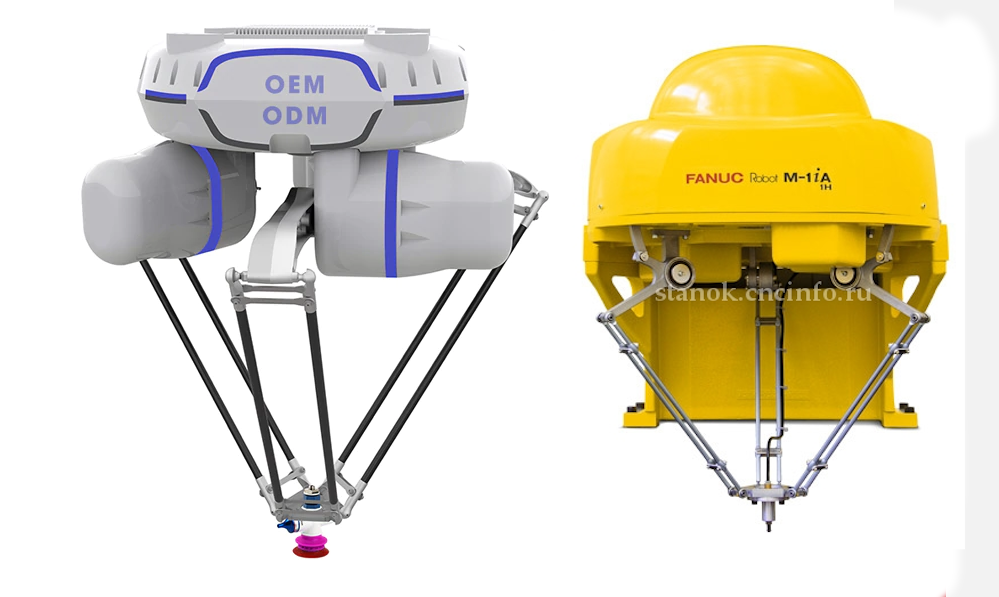
\includegraphics[width=0.8\linewidth]{./image/odm}
\caption{Примеры конкурентов на рынке}
\end{figure} 

Робот <<OEM ODM>> китайского происхождения, стоит 744 тыс. рублей, но без представительства в России. Робот <<Fanuc>> японского происхождения, но собирается в России. Стоимость зависит от заказчика, мне удалось выяснить, что начинается она от 600 тыс. руб. Оба робота имеют грузоподьемность в килограмм, высокую точность позиционирования, и массивную базу. У <<Fanuc>> база весит 17 кг., позволяя ему избегать вибраций, возникающих при работе. Данные роботы предназначены для чистых производств, маловероятно увидеть их на сортировке мусора. Ниша сверхдешёвых дельта-роботов на данный момент свободна, что связано со сложностью написания программного обепечения для управления паралельной машиной.

Сбывать продукцию следуют среди фирм не желающих тратить больших средств на механизацию ручного труда. Там, где именитые фирмы не могут предложить свои услуги из-за завышенных цен изделия, можно предложить замену, способную конкурировать с низкооплачиваемым человеческим трудом. Мусороперерабатывающие заводы, небольшие фабрики пищевого производства. 

\subsubsection{Ценовая политика}

Основной статьей заработка следует считать разработку программного продукта для решения конкретной задачи, поставленной заказчиком. Так как свободное ПО для управления данным типом робота отсутсвует в принципе, программы придется писать в любом случае. Особенно в начале, когда не будет еще большого опыта и наработанной базы проектов. Поэтому за программый продукт логично брать больше, чем стоимость самого робота, более того, возможно, передать электроннные модели закачику.

\subsubsection{Сбытовая политика и мероприятия}
\begin{table}[h!]
    \centering
\begin{tabular}{|l|c|c|c|c|c|}
\hline
Показатели &\multicolumn{4}{|c|}{Квартал}   & Всего\\
\hline
           & I & II & III & IV & \\ 
\hline
\textbf{Разработка ПО}  & &  &  &  &  \\
\hline
Ожидаемы объем продаж, ед.  & 1  & 2  & 2  & 3  & 8  \\
\hline
Цена с НДС, т.р.  & 300  & 300  & 300  & 300  &  \\
\hline
Выручка с НДС, т.р.   & 300  & 600  & 600  & 900  & 2400 \\
\hline
Нетто-выручка (без НДС), т.р.  & 250   & 500  & 500  & 750  & 2000 \\
\hline
Сумма НДС, т.р   & 50  & 100 & 100  & 150  & 400 \\
\hline
\textbf{Дельта-робот}  & &  &  &  &  \\
\hline
Ожидаемы объем продаж, ед.  & 3 & 6  & 9  & 18  & 36  \\
\hline
Цена с НДС, т.р.  & 50  & 50  & 50  & 50  &  \\
\hline
Выручка с НДС, т.р.   & 150  & 300 & 450  & 900  & 1800 \\
\hline
Нетто-выручка (без НДС), т.р.  & 125  & 250  & 375  & 750  & 1500 \\
\hline
Сумма НДС, т.р   & 25   & 50  & 75  & 150  & 300 \\
\hline
\end{tabular}
\caption{План продаж}
\end{table}



\subsection{План производства}
                            
Группы комплектующих, из которых будет состоять система:\\
1) Комплектующие которые печатаются на 3д принтере: основные конструкционные детали, редуктор, шарниры, крепление, каретка и части рабочего органа.\\
2) Электроника, включающая в себя arduino cnc shield, драйвера двигателей A4988, шаговые двигатели, orange Pi, orange Pi camera, импульсный адаптер питания, концевики.\\
3) Силовые элементы, в качестве которых выступает квадратная алюминеевая труба 15х15 мм. и круглая алюминиевая труба 8 мм. В зависимости от требований заказчика, диаметры труб можно варьировать.\\
4) Прочие расходные материалы: подшипники, винты, самоконтрящиеся гайки, провода, стяжки.

Основной процесс изготовления заключен в печати деталей базы, последующей механической обработке (снятие поддержек, ошкуривание и подобное) и самого процесса сборки. Для печати выбран пластик PetG, как самый распространенный пластик, имеющий неплохие прочностные характеристики, не разлагающийся под действием ультрафиолета и работающего при температурах до $80^{\circ} C$. Конечно, возможен переход на промышленные пластики, показатели которых на совершенно ином уровне. Но это приведет к необходимости изменить геометрию деталей, сделать их более грацильными, так как во многих местах прочность будет излишняя.

\begin{table}[h!]
    \centering
\begin{tabular}{|l|c|c|c|c|c|}
\hline
Модель stl &  Время печати & Штук  & Расход г. & Общее время & Общий расход\\
\hline
basa  &  12h 58m & 1 & 132.77 & 12h 58m & 132.77 \\
\hline
krepej  &  11h 10m & 3 & 96.68 & 1d 9h 30m & 290.04\\
\hline
worm  &  3h 35m & 3 & 31.74 & 10h 45m & 95.22 \\
\hline
ploshadka1  &  3h 1m & 1 & 24.47 & 3h 1m & 24.47\\
\hline
ploshadka2  &  2h 53m & 1 & 24.21 & 2h 53m & 24.21\\
\hline
krep\_konch\_niz  &  31m & 3 & 3.92 & 1h 33m & 11.76\\
\hline
krep\_konch  &  30m & 3 & 3.97 & 1h 30m & 11.91\\
\hline
lokot\_verh  &  2h 18m & 3 & 24.18 & 6h 54m  & 72.54\\
\hline
lokot\_niz  &  37m & 12 & 6.68 & 7h 24m & 80.16\\
\hline
plecho\_krep  & 1h 26m & 3 & 11.56 & 4h 18m & 34.68\\
\hline
Итого:  &  &  &  & 3d 12h 46m & 777.76\\
\hline
\end{tabular}
\caption{Расход времени и пластика на печать деталей}
\end{table}

Время, приведенное в таблице 1, отображает минимальное время требуемое для печати, без учета времени на разогрев, постановку на печать следующей детали и возможных прерываний печати, связанных с застреванием филамента, плохой адгезией или сдвигом по слоям. Для достижния приемлеммых временных рамок, требуется использовать параллельную печать, минимум на 2 принтерах. При получении крупного заказа, выполнить его в разумные сроки будет возможно только при создании фермы из принтеров. 

\begin{table}[h!]
    \centering
\begin{tabular}{|l|c|c|c| }
\hline
Наименование & Штук & Цена за шт. руб.  & Стоимость руб. \\
\hline
Arduino Uno & 1 & 300 & 300 \\
\hline
Arduino CNC Shield & 1  & 250 & 250 \\
\hline
driver A4988 & 3  & 100 & 300 \\
\hline
Адаптер питания 500 Вт. & 1 & 1250 & 1250 \\
\hline
Orange Pi  с камерой & 1 & 1400 & 1400\\
\hline
Двигатели Nema 17 & 3  & 475  & 1425  \\
\hline
Концевой переключатель & 6 & 10  & 60  \\
\hline
Подшипник 5х8х2.5 & 6  & 32  &  192 \\
\hline
Труба квадратная 15х15 мм. 2м. & 1  & 200  & 200  \\
\hline
Труба круглая 8 мм. 1м & 2 & 80 & 160 \\
\hline
Винты и прочий крепеж & 1 & 300 & 300 \\
\hline
Филамент PetG кг.  &  1  & 1300 & 1300 \\
\hline
Итого: &  &  & 7137 \\
\hline
\end{tabular}
\caption{Стоимость расходников}
\end{table}

Под производства необходимо два помещения: офисное для проектирования и мастерская для сборки и печати. В офисе необходимо два компьютера:

- для менеджера по продажам и закупкам продукции

- рабочее место проектировщика с CAD-приложением, слайсером для 3d печати.

В мастерской необходимы:

- место электрика, оборудованное паяльными принадлежностями, набором коробок и стеллажей для комплектующих.

- верстак с рабочими инструментами, где можно будет скручивать соединения, обрабатывать детали, проводить сборку.

- место для размещения 3д принтеров.

Минимальная цена аренды промышленного помещения в 50 м.$^{2}$ в Санкт-Петербурге стоит около 40 тыщ. рублей в месяц. 480 тыщ. рублей в год.
\begin{table}[h!]
\centering
\begin{tabular}{|l|c|c|c|}
    \hline
    Наименование & Штук & Цена тыщ. руб.  & Стоимость тыщ. руб. \\
    \hline
    Автоматизированное рабочее место & 2 & 80  & 160 \\
    \hline
    3д принтер & 2 & 50  & 100 \\
    \hline
    Рабочее место электрика & 1 & 100 & 100 \\
    \hline
    Верстак с инструментом & 1 & 100 & 100 \\
    \hline
    Итого: &&& 420 \\
    \hline
\end{tabular}
\caption{Стоимость оборудования}
\end{table}

Основным процессом производства будет проектирование деталей, для реализации пожеланий заказчика и печать деталей. С двумя принтерами изготовление комплекта для одного робота должно укладываться в рабочее время 5-6 календарных дней. Разброс неизбежен, так как время зависит от размеров итоговых деталей. Для реализации большого заказа необходимо докупать дополнительные принтеры, либо отдавать печать на оутсорс в ателье 3д печати, что может рассматриваться, как очень выгодный вариант.

По моему мнению, необходимый персонал может состоять из двух человек, каждый из которых берет на себя сразу по две роли. Конечно, роли поделены достаточно условно, каждый должен быть готов подменить другого и понимать работу товарища.  

\begin{table}[h!]
\centering
\begin{tabular}{|l|c|c|c|}
    \hline
    Наименование & Ставка & Зарплата тыщ. руб.& Всего тыщ. руб. \\
    \hline
    Инженер проектировщик & 0.5 & 80  & 40 \\
    \hline
    Оператор 3д принтера & 0.5 & 50  & 25 \\
    \hline
    Электрик-сборщик & 0.5 & 50 & 25 \\
    \hline
    Менеджер по продажам & 0.5 & 50 & 25 \\
    \hline
    Итого зарплата в месяц: &&& 105 \\
    \hline
\end{tabular}
\caption{Первоначальный уровень зарплат}
\end{table}


\subsection{Финансовый план}

\begin{longtable}[c]{|p{110pt}|p{110pt}|c|c|c|c|c|}
\hline
Показатели & Источник информации  &\multicolumn{4}{|c|}{Квартал}   & Всего\\
\hline
& & I & II & III & IV & \\ 
\hline
1. Вырочка-нетто (без учета НДС) от реализации & План продаж  & 450 & 900  & 1050  & 1800  & 4200  \\
\hline
2. Переменные производственные затраты &  &  &  &  &  &  \\
\hline
2.1 Переменные материальные затраты & План материально-производственных затрат  & 21.411 & 42.822  & 64.233  & 128.466  & 256.932  \\
\hline
2.2 Переменные затраты на оплату труда & План затрат на оплату труда производственного персонала   & 315 & 315 & 315 & 315 & 1260 \\
\hline
2.3 Переменные общепроизводственные затраты  & План общепроизводственных затрат  & 540 & 120  & 120  & 120  & 480 \\
\hline
3. Валовая прибыль &  & 428.589 & 857.178  & 985.767 & 1671.534 & 4943.068  \\
\hline
4. Переменные управленческие и коммерческие затраты & План управленческих и коммерческих затрат  & 0  & 0  & 0 & 0 & 0 \\
\hline
5. Маржинальная прибыль &  &  &  &  &  &  \\
\hline
5.1 Разработка ПО  &   & 250  & 500  & 500 & 750  & 2000 \\
\hline
5.2 Дельта-робот &  & 103.589  & 257.178 & 385.767 & 771.534 & 1543.063  \\
\hline
6.1 Постоянные общепроизводственные затраты  & План общепроизводственных затрат  & 75  & 150 & 175  & 300  & 700  \\
\hline
6.2 Постоянные управленческие и коммерческие затраты & План управленических и коммерческих затрат  & 0 & 0 & 0 & 0 & 0 \\
\hline
7. Прибыль от продаж &  & 375  & 750 & 875  & 1500 & 3500  \\
\hline
8. Прибыль до налогооблажения & & 450  & 900 & 1050  & 1800  & 4200  \\
\hline
9. Налог на прибыль &  & 75  &  150  &  175 & 300 & 700 \\
\hline
10. Чистая (нераспределенная) прибыль &  & -626.411  & 422.178 & 550.767 & 1236.534 & 1583.068\\
\hline
\caption{Финансовый план}\label{long}

\end{longtable}


Расчет показателя NPV.\\

$NPV = \frac{-206.411+422.178+550.767+1236.534}{1.1}-420-480= 820,97$\\

Так как NPV получился положительным, значит финансирование проекта является целесобразным.




% заключение
\addcontentsline{toc}{section}{Заключение}
\begin{center}
\large{\textbf{ЗАКЛЮЧЕНИЕ}}\\
\end{center}
Бла-бла-бла просто гений

% список источников
\addcontentsline{toc}{section}{Список}
\begin{center}
\large{\textbf{СПИСОК ИСПОЛЬЗОВАННЫХ ИСТОЧНИКОВ}}\\
\end{center}
1. какая-то статья 


% приложения (не обязательно)
\end{document}
